% DO NOT COMPILE THIS FILE DIRECTLY!
% This is included by the other .tex files.

\begin{frame}[t,plain]
\titlepage
\end{frame}

\begin{frame}
    \frametitle{Content of the presentation}
    \begin{itemize}
        \item What problems are we trying to tackle
        \item MISP Workflows overview
        \item Design of the system \& how can it be extended
    \end{itemize}
\end{frame}

\begin{frame}
    \frametitle{What problems are we trying to tackle}
    \begin{itemize}
        %\item Initial idea came from GeekWeek7.5\footnote{Workshop organized by the Canadian Cyber Center}{https://cyber.gc.ca/en/events/geekweek-75}
        \item Initial idea came from GeekWeek7.5\footnote{\href{https://cyber.gc.ca/en/events/geekweek-75}{Workshop organized by the Canadian Cyber Center}}
        \begin{center}
            
\includegraphics[width=0.3\linewidth]{pictures/geekweek75.jpg}
        \end{center}
        \item Experienced users wanted to be able to interact with the behavior of MISP for specific operations
        \item Same spirit than web-hooks but more flexible
        \item Use-cases:
        \begin{itemize}
            \item Prevent publication of events not meeting some criterias
            \item Enrich events before the actual publication takes place
            \item Prevent querying thrid-party service (e.g. virustotal) for sensitive information
            \item Send a notification in chat room when new events get published
            \item And much much more..
        \end{itemize}
    \end{itemize}
\end{frame}

\begin{frame}
    \frametitle{Simplistic overview}
    \begin{enumerate}
        \item \textbf{User Interacts} with MISP using the UI or API
        \item MISP handles the request, starts \textbf{preparing data} to perform the operation
        \item MISP checks if there is an enabled workflow \textbf{listening to the trigger}
        \item MISP fetches enabled workflows and \textbf{executes} them
        \item If all went fine, MISP \textbf{continue} to perform the operation
        \begin{itemize}
            \item The operation can potentially be cancelled by \texttt{blocking} modules
        \end{itemize}
    \end{enumerate}
\end{frame}

\begin{frame}
    \frametitle{Terminology}
    \begin{enumerate}
        \item \textbf{workflow}: Sequence of actions to be executed
        \item \textbf{execution path}: A path composed of actions to be executed sequentially
        \begin{itemize}
            \item A workflow can contain more than one execution path
        \end{itemize}
        \item \textbf{trigger}: Starting point of an \texttt{execution path}. Triggers are called when specific actions are done by MISP
        \begin{itemize}
            \item A trigger can only have one workflow and vice-versa
        \end{itemize}
    \end{enumerate}
    \begin{center}
        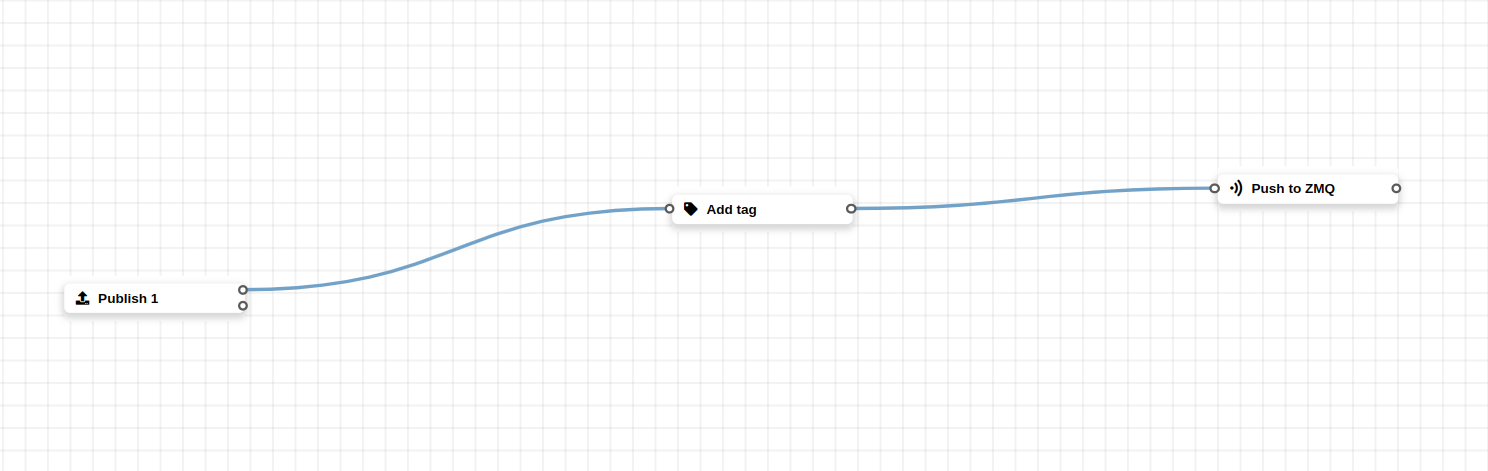
\includegraphics[width=1.0\linewidth]{pictures/workflow-view.png}
    \end{center}
\end{frame}

\begin{frame}
    \frametitle{Workflow execution}
    \begin{enumerate}
        \item An operation happen in MISP (e.g. event publication)
        \item A trigger is called
        \item Collect enabled workflow listening to called trigger
        \item Execute workflow
        \begin{itemize}
            \item \texttt{\color{green!50!black}success}: Proceed with the operation
            \item \texttt{\color{red}failure} | \texttt{\color{blue}cancel}: Cancel the operation
        \end{itemize}
    \end{enumerate}
\end{frame}

\begin{frame}
    \frametitle{Execution Paths}
    Currently 2 types of execution path:
    \vspace{0.5em}
    \begin{itemize}
        \item {\bf Blocking}: Execution is stoped in case of error or module cancel
        \begin{itemize}
            \item Current workflow's blocking execution path is {\bf stopped}
        \end{itemize}
        \vspace{0.5em}
        \item {\bf Non-blocking/Parallel}: Stop execution for current path only
        \begin{itemize}
            \item Current execution path is {\bf stopped}
            \item {\bf Resume} execution of remaining paths
        \end{itemize}
    \end{itemize}
\end{frame}

\begin{frame}
    \frametitle{Publishing example}
    Example:
    \begin{enumerate}
        \item An Event is published
        \item MISP starts the publishing process
        \item MISP executes the workflow listening to the trigger
        \begin{itemize}
            \item {\bf\color{green!50!black}success execution success}: Proceed publishing
            \item {\bf\color{red}success execution failure}: Stop publishing, log the reason and report the failure back to the user
        \end{itemize}
    \end{enumerate}
\end{frame}

\begin{frame}
    \frametitle{Execution context}
    \begin{itemize}
        \item Workflow are \textit{triggered by any users}
        \item However, the user for which the workflow executes has the \texttt{site-admin} role and is from the \texttt{MISP.host\_org\_id}
        \item This is to make sure, all data are processed regardless of the ACL
    \end{itemize}
\end{frame}

\begin{frame}
    \frametitle{Workflow modules}
    \begin{center}
        
\includegraphics[width=0.5\linewidth]{pictures/module-type.png}
    \end{center}
    4 types of module
    \begin{itemize}
        \item \textbf{logic}: Allow to redirect the execution flow.
        \begin{itemize}
            \item IF condition, fork the blocking execution into a non-blocking one, ...
        \end{itemize}
        \item \textbf{action}: Can modify data, prevent execution or perform additional actions
        \begin{itemize}
            \item Publish to ZMQ, perform enrichments, block the execution, ...
        \end{itemize}
        \item \textbf{misp-module}: Basically \texttt{action} modules but using the \texttt{misp-module} service for the logic
        \begin{itemize}
            \item Written in Python!
        \end{itemize}
        \item \textbf{custom}: Allow user to create their own \texttt{action} and \texttt{logic} module in PHP
        \begin{itemize}
            \item Can use any functions defined in the application
        \end{itemize}
    \end{itemize}
\end{frame}

\begin{frame}
    \frametitle{Workflow modules}
    \texttt{action} modules can be from 3 sources
    \begin{itemize}
        \item \texttt{\scriptsize app/Model/WorkflowModules/action/[module\_name].php}
        \begin{itemize}
            \item Built-in module in the application
            \item Written in PHP
            \item Can use MISP's built-in functionalities (restsearch, enrichment, push to zmq, ...)
            \item Fast and easier to interact with for those having internal knowledge of MISP
        \end{itemize}
        \item \texttt{\scriptsize app/Lib/WorkflowModules/action/[module\_name].php}
        \begin{itemize}
            \item Same as previous but allow users to create their own without sharing with the community
        \end{itemize}
        \item \texttt{From the misp-module service} 
        \begin{itemize}
            \item Written in Python
            \item Can use any python libraries
            \item New \texttt{misp-module} module type: \texttt{action}
        \end{itemize}
    \end{itemize}
    \begin{center}
        $\rightarrow$ Both the PHP and Python systems are \textbf{plug-and-play}
    \end{center}
\end{frame}

\begin{frame}
    \frametitle{Getting started with workflows (1)}
    Review MISP settings:
    \begin{enumerate}
        \item Make sure \texttt{MISP.background\_jobs} is turned on
        \item Turn on setting \texttt{Plugin.Workflow\_enable}
        \item Make sure workers are up-and-running
    \end{enumerate}
    \begin{center}
        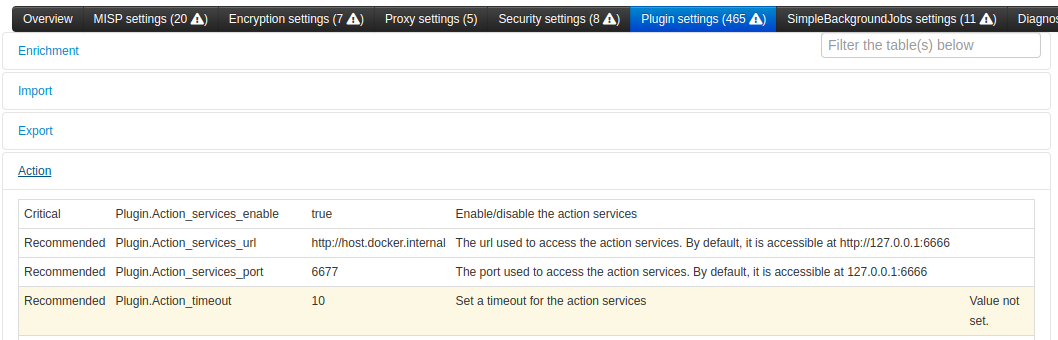
\includegraphics[width=0.75\linewidth]{pictures/settings-1.png}
        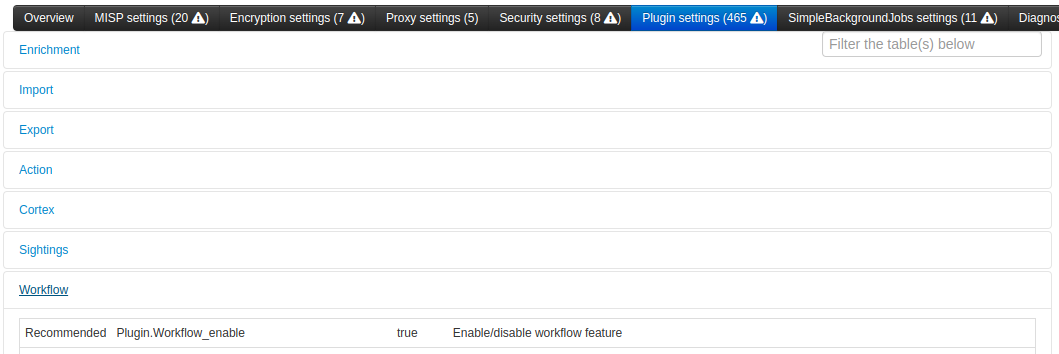
\includegraphics[width=0.75\linewidth]{pictures/settings-2.png}
    \end{center}
\end{frame}

\begin{frame}
    \frametitle{Getting started with workflows (2)}
    If you wish to use action modules from the \texttt{misp-module}:
    \begin{itemize}
        \item Make sure you update your \texttt{misp-module} application to the latest version
        \item Make sure your have the new \texttt{action\_mod} module type in \url{misp-modules/misp\_modules/modules}
        \item Restart your \texttt{misp-module} application
    \end{itemize}
\end{frame}

\begin{frame}
    \frametitle{Getting started with workflows (3)}
    \begin{enumerate}
        \item Go to the trigger list: \texttt{Administration > Workflows}
        \begin{itemize}
            \item \url{/workflows/triggers}
        \end{itemize}
        \item Turn a trigger on
        \item Use the editor to edit the workflow associated to this trigger
    \end{enumerate}
\end{frame}

\begin{frame}
    \frametitle{Creating a workflow with the editor}
    \begin{enumerate}
        \item Choose a \texttt{trigger} from the list
        \item Drag an \texttt{action} module from the side panel to the canvas
        \item From the \texttt{trigger} output, drag an arrow into the \texttt{action} input (left side)
    \end{enumerate}
    \begin{center}
        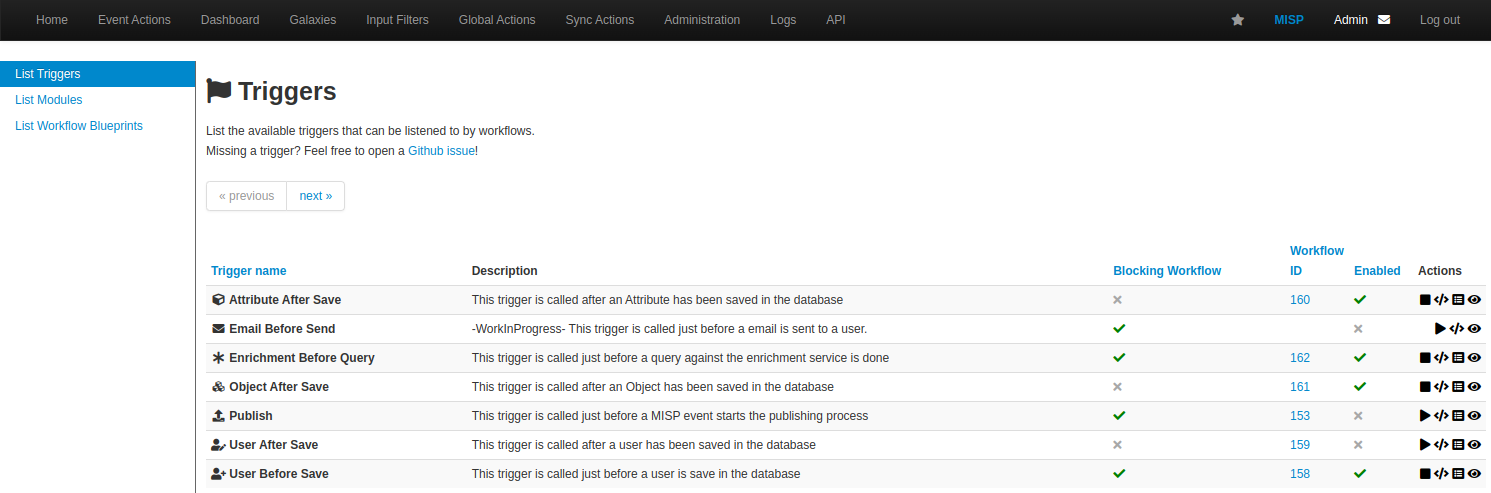
\includegraphics[width=0.8\linewidth]{pictures/usage-1.png}
    \end{center}
    \begin{center}
        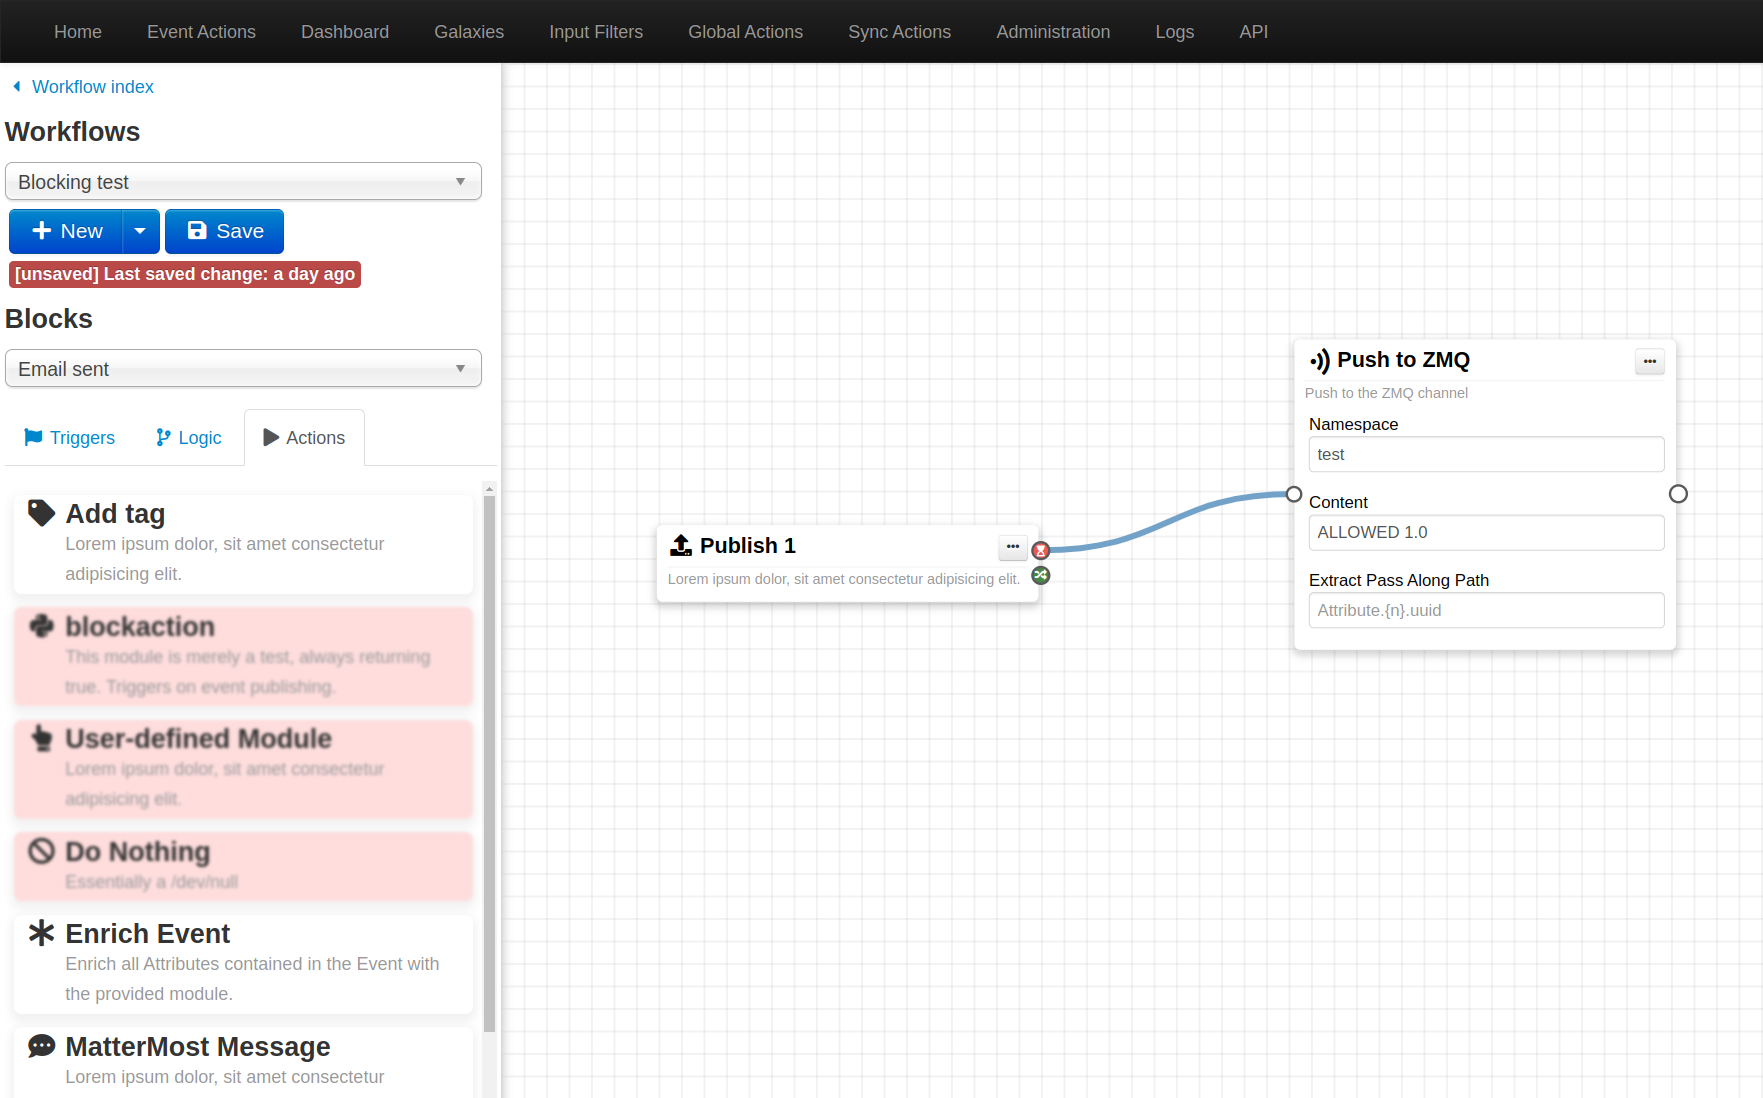
\includegraphics[width=0.50\linewidth]{pictures/editor-1.png}
    \end{center}
\end{frame}

\begin{frame}
    \frametitle{Working with the editor}
    Operations not allowed:
    \begin{itemize}
        \item Execution loop are not authorized
        \begin{itemize}
            \item Current caveat: If an action re-run the workflow in any way
        \end{itemize}
    \end{itemize}
    \begin{center}
        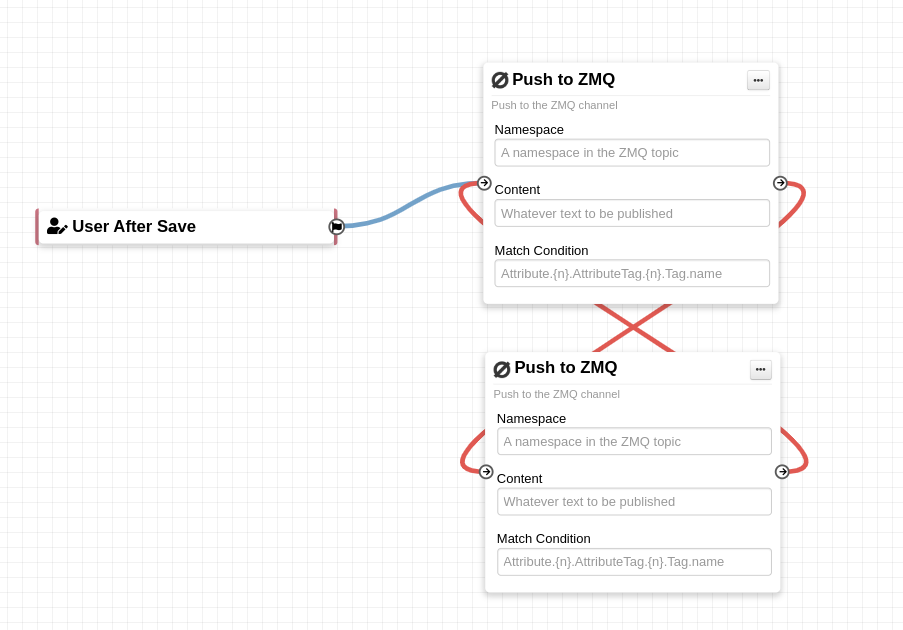
\includegraphics[width=0.7\linewidth]{pictures/editor-not-allowed-1.png}
    \end{center}
\end{frame}

\begin{frame}
    \frametitle{Workflow blueprints: Create}
    Select one or more modules to be saved as blueprint then click on the \texttt{save blueprint} button
    \begin{center}
        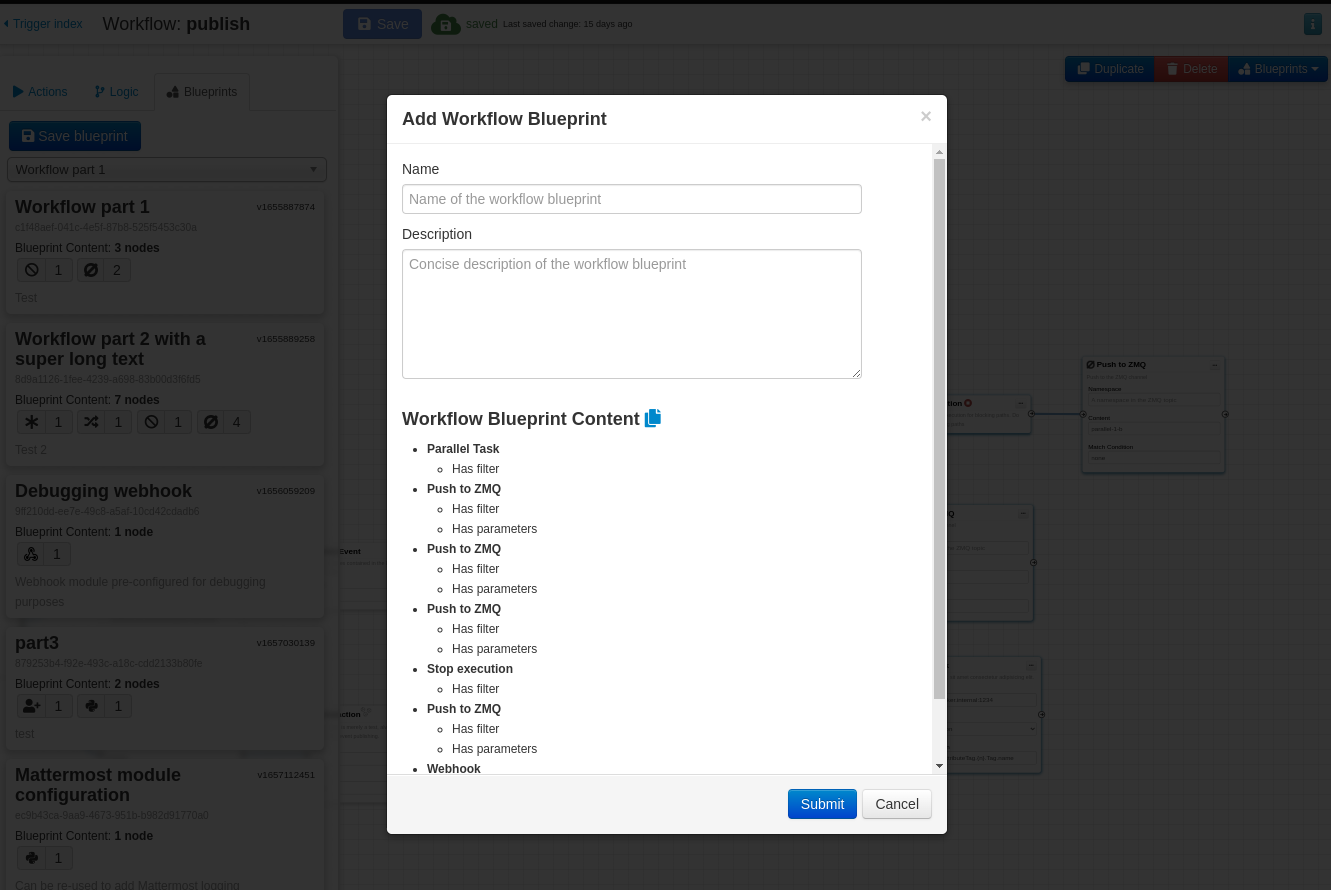
\includegraphics[width=0.85\linewidth]{pictures/blueprint-1.png}
    \end{center}
\end{frame}

\begin{frame}
    \frametitle{Module filtering}
    \begin{itemize}
        \item Some action module accept \texttt{module filtering} conditions
        \item For example, the \texttt{enrich-event} module will only perform the enrichment on Attribute having a \texttt{tlp:white} tag
    \end{itemize}
    \begin{center}
        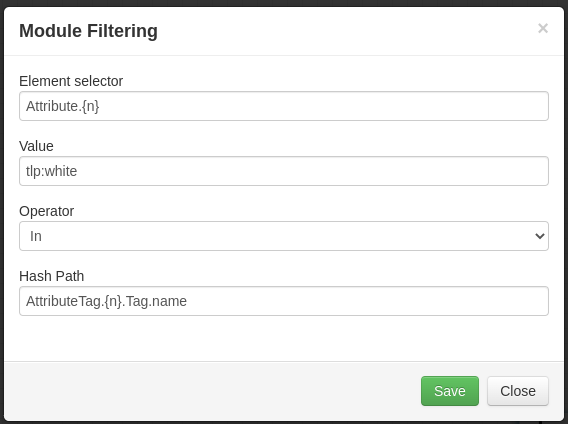
\includegraphics[width=0.7\linewidth]{pictures/module-filtering.png}
    \end{center}
\end{frame}

\begin{frame}
    \frametitle{TODOs / FIXMEs}
    \begin{enumerate}
        \item Show which workflows use a module and the other way around
        \item Perfom parallel execution by a worker (currently in-line)
        \item Implement parallel task module
        \item ACL-aware: new \texttt{workflow editor} role
        \item Standardize how data is passed between modules
    \end{enumerate}
\end{frame}

\section{Learning by examples}
\begin{frame}
    \frametitle{Workflow example 1}
    \begin{center}
        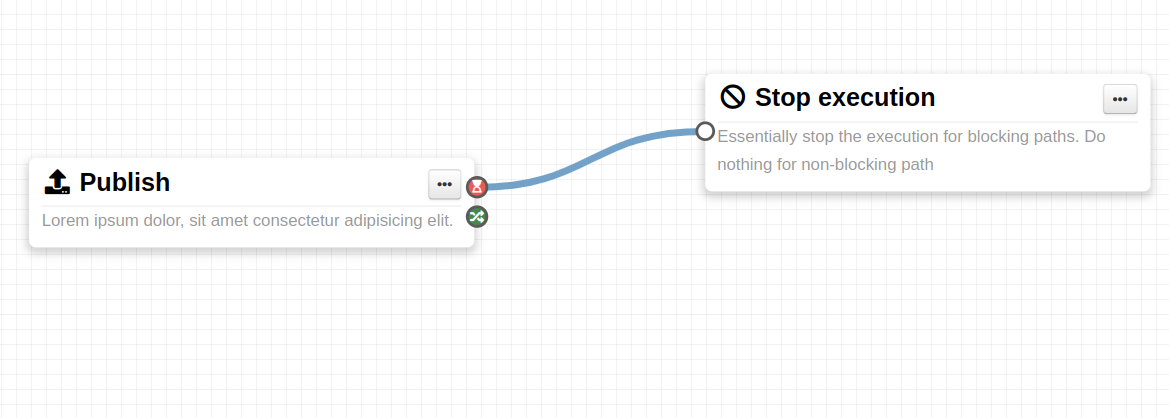
\includegraphics[width=0.95\linewidth]{pictures/example-1.png}
    \end{center}

    \begin{itemize}
        \item The \texttt{zmq} module will be run if at least one of the attribute has the \texttt{tlp:white} tag.
    \end{itemize}
\end{frame}

\begin{frame}
    \frametitle{Workflow example 2}
    \begin{center}
        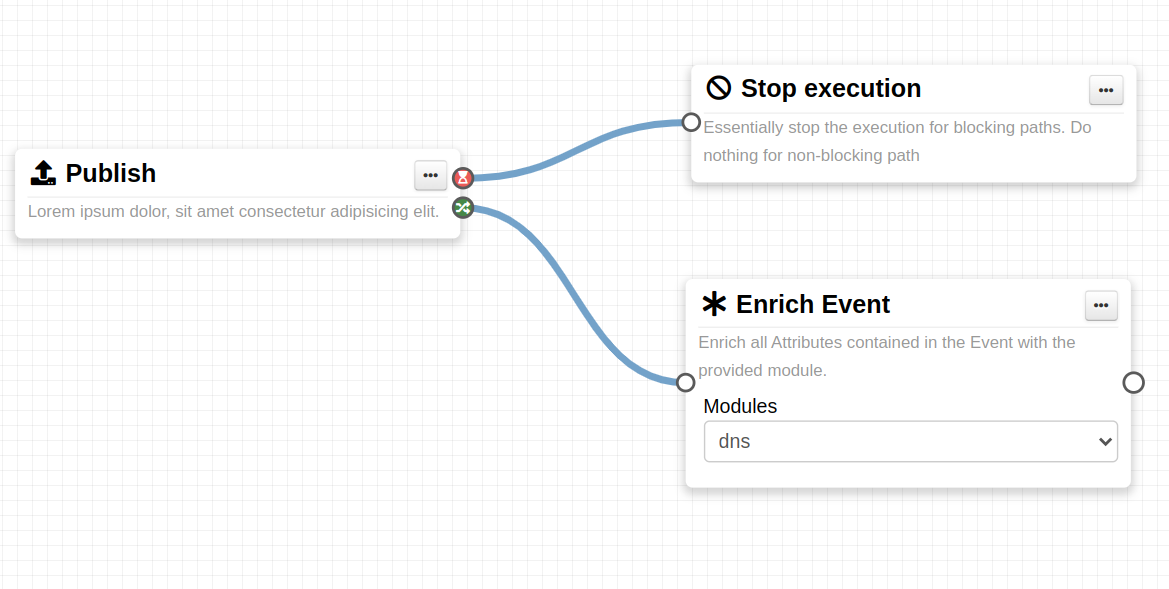
\includegraphics[width=0.95\linewidth]{pictures/example-2.png}
    \end{center}

    \begin{itemize}
        \item If an event has the \texttt{PAP:RED} tag or any of the attribute has it, the enrichment process will be cancelled
    \end{itemize}
\end{frame}

\begin{frame}
    \frametitle{Workflow example 3}
    \begin{center}
        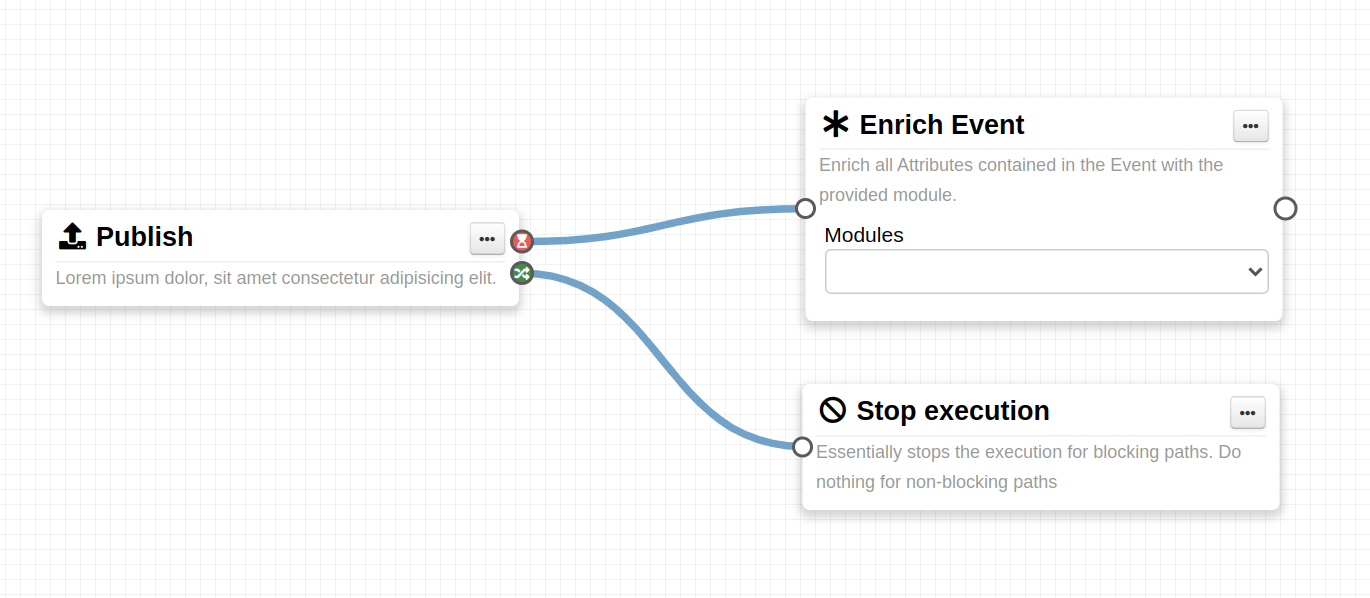
\includegraphics[width=0.65\linewidth]{pictures/example-3.png}
    \end{center}

    \begin{itemize}
        \item After a user has been saved, a message containing the user's email will be sent to a Mattermost channel and the user detailed will be posted to the webhook URL
    \end{itemize}
\end{frame}

\begin{frame}
    \frametitle{Creating a new module in PHP}
    \begin{center}
        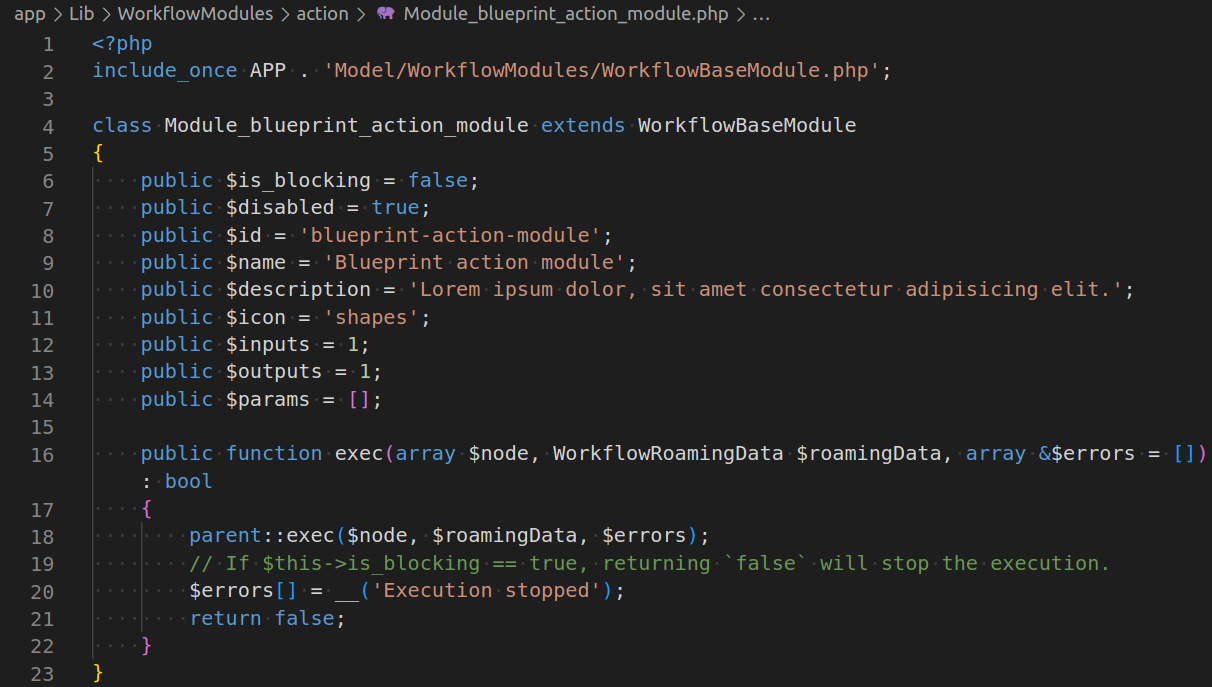
\includegraphics[width=0.65\linewidth]{pictures/custom-1.png}
    \end{center}

    \begin{itemize}
        \item Module configuration are defined as public variables
        \item The \texttt{exec} function has to be implemented.
        \begin{itemize}
            \item If it returns \texttt{true}, execution will proceed
            \item If it returns \texttt{false}
            \begin{itemize}
                \item And the module is \texttt{blocking}, the execution will stop and the operation will be blocked
                \item And the module is not \texttt{blocking}, the execution for the current path will stop
            \end{itemize}
        \end{itemize}
    \end{itemize}
\end{frame}


\begin{frame}
    \frametitle{Creating a new module in Python}
    \begin{center}
        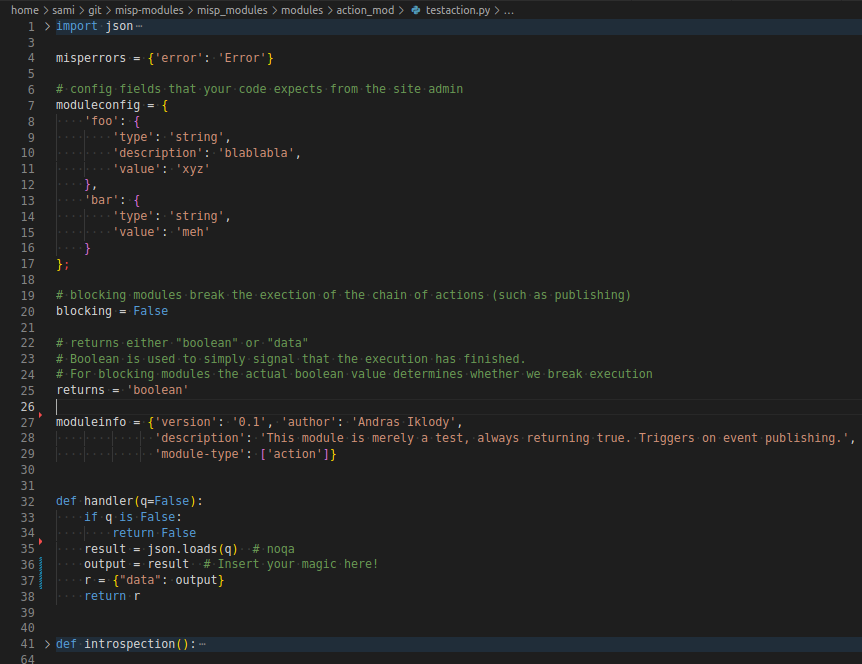
\includegraphics[width=0.6\linewidth]{pictures/custom-2.png}
    \end{center}

    \begin{itemize}
        \item Module configuration are defined in the \texttt{moduleinfo} and \texttt{moduleconfig} variables
        \item The \texttt{handler} function has to be implemented.
        \item Blocking logic is the same as other modules
    \end{itemize}
\end{frame}

